%
% Catam project simulating wind forced ocean currents
%
\documentclass{article}
\usepackage{amsmath}
\usepackage{empheq}
\usepackage{graphicx}
\usepackage{bm}
\usepackage{framed}
\usepackage{enumerate}
\usepackage{array}
%\usepackage{pgfplots}
\usepackage{caption}
\usepackage{amsfonts}
\usepackage[margin=3cm]{geometry}
\usepackage{float}

\begin{document}

\title{Dynamical Systems}
\author{Course given by Prof. J.Lister \\
\LaTeX\  by Dominic Skinner \\
Dom-Skinner@github.com}
\maketitle
\section*{Introduction}
A dynamical system is a set of equations describing the evolution of a system
with respect to a time-like variable. Usually they are non-linear.
\\
The possible states of the system define the state space/phase space.
\\
\\
\textbf{Example:}   The logistic map
\[ x_{n+1} = \mu x_n ( 1- x_n) \]
For $ 0 \leq \mu \leq 4 $ this describes evolution with respect to a discrete time 
$n$ in a state space $[0,1]$.
\\
\\
\textbf{Example:}   The Lotka-Voltera equations
\begin{align*}
\dot{r} &= r(a - br -cs) \\
\dot{s} &= s(d - er -fs)
\end{align*}
Where \emph{a-f} are positive constants. These describe continous evolution 
in a state space $(r,s) \in [0 , \infty] \times [0, \infty]$ as a model for 
the population of two species competing for the same food supply.
\\
\\
\textbf{Example:}   The non-linear Schr\"odinger equation
\[ i \frac{\partial \Psi}{ \partial t} = \nabla^2 \Psi + |\Psi|^2 \Psi \]
This describes evolution in an infinite dimensional statespace of possible
wavefunctions.
\\
\\
Because the equations are non-linear, it is often impossible to find a complete
set of closed form analytic solutions. Instead, we resort to a mixture of 
geometric and analytic arguments, and aim to say something about the generic
long-term behaviour.
\\
\\
\textbf{Example:}   
\begin{align*}
\dot{r} &= r(3 - r -s) \\
\dot{s} &= s(2 - r -s)
\end{align*}
Consider the regions where $\dot{r}$ and $\dot{s}$ are $>0, \; <0, \; =0$. 
\\
If $r,s >0$ then
\begin{align*}
r+s &< 2 \implies \dot{r}, \dot{s} > 0 \\
2 < r+s &< 3 \implies \dot{r} >0 , \; \dot{s} < 0 \\
r+s &> 3 \implies \dot{r}, \dot{s} < 0 \\
\end{align*}
$\dot{r} = 0$ if $r=0$ or $r+s = 3$. \\
$\dot{s} = 0$ if $s=0$ or $r+s = 2$. \\
Therefore $\dot{r} = \dot{s} = 0$ at the fixed points $(0,0), \; (3,0), \; (0,2)$.
This gives the phase portrait/diagram/plane%
\footnote{Phase portrait, phase diagram, phase plane will be used interchangably}
% INCLUDE GRAPHIS HERE
\begin{figure}[H]
\centering
\includegraphics[width=4cm, height=4cm]{fig0.png}
\end{figure}
The most important feature of the phase portrait is that all solutions with 
$r >0$ tend to the stable fixed point $(3,0)$. The fixed points $(0,0)$ and
$(0,2)$ are unstable. There are no periodic orbits.
\\
\\
\textbf{Example:}   
\begin{align*}
\dot{r} &= r(3 - r -s) \\
\dot{s} &= s(2 - \mu r -s)
\end{align*}
In this case, a new fixed point $(\frac{1}{1- \mu} , \frac{2 - 3 \mu}{1- \mu})$
appears in the state space at $\mu = \frac{2}{3}$ and for $\mu < \frac{2}{3}$ 
is the long term stable attractor. 
\\
A qualitative change in the solution structure is called a bifurcation.
\\
\\
\textbf{Example:}   
\begin{align*}
\dot{x} &= -y + \epsilon x (\mu - x^2 - y^2) \\
\dot{y} &= \;\;\; x + \epsilon y (\mu - x^2 - y^2)
\end{align*}
Use polar coordinates which are a more natural choice for this problem.
In general:
\begin{empheq}[box=\fbox]{align}
\dot{r} &= \frac{x \dot{x} + y \dot{y}}{r} \nonumber \\
\dot{\theta} &= \frac{x \dot{y} - y \dot{x} }{ r^2} \nonumber
\end{empheq}
Which are equations that will be referred to frequently. \footnote{so learn them now!}
In our example, they become
\begin{align*}
\dot{r} &= \epsilon r (\mu - r^2) \\
\dot{\theta} &= 1
\end{align*}
Consider $\dot{r}$ and $\dot{\theta}$:
% INSERT DIAGRAM HERE
\begin{figure}[H]
\centering
\includegraphics[width=8cm, height=6cm]{fig1.png}
\end{figure}
The infinite set of periodic solutions for $\epsilon = 0$ is destroyed by any 
perturbation to $\epsilon \neq 0$. This is an example of structural instability.
If $\mu > 0$ then just one limit cycle survives and is stable (unstable) for 
$\epsilon >0$ ($\epsilon < 0$). The appearance of the limit cycle as $\mu \uparrow$ 
through $0$ is another form of bifurcation.
\\
\\
\textbf{Example:} In 2D the points of successive interection $x_n$ of a 
solution near a limit cycle with a line $\varepsilon$ perpendicular to the cycle,
move monotonically towards/away from the point of intersection $x^{*}$ of 
$\varepsilon$ with the limit cycle.
% INSERT PLOT HERE
\begin{figure}[H]
\centering
\includegraphics[width=7cm, height=4cm]{fig2.png}
\end{figure}
The point $x^{*}$ is a stable/unstable fixed point of this Poincar\'e recurrence
map.
\\
In 3 or higher dimensions, or in 2D with time-dependent coefficients there is 
room for much more complicated behaviour including \underline{chaos}.
%%%%%%%%%%%%%CHAPTER 1
\section{Basic Definitions}
We need some termonology.
\subsection{Notation}
We only consider ODEs of the form 
\begin{equation}\tag{*}
\dot{\textbf{x}} = \textbf{f(x)}
\end{equation}
for \textbf{x} in a phase space/state space $E \subset \mathbb{R}^{n}$.
The n first order ODEs form a dynamical system of order (dimension) n.
\\
\\
Since
\[ \frac{\partial \textbf{f} } { \partial t} = 0 \]
 we call the system \underline{autonomous}.
\\
\\
A non-autonomous system $\dot{\textbf{x}} = \textbf{f}(\textbf{x} ,t) $ can be
made autonomous by setting
\[ \textbf{y} = ( \textbf{x},t) \quad \mbox{ with } \quad \dot{\textbf{y}} = ( \textbf{f}(\textbf{y}),1) \]
The n$^{th}$ order ODE
\[ \frac{d ^n x}{d t^n} = g \left( x , \frac{d x}{d t} , \dots , \frac{d^{n-1} x}{d t^{n-1}} \right) \]
can be put in the form (*) by setting
\[ \textbf{y} =  \left( x , \frac{d x}{d t} , \dots , \frac{d^{n-1} x}{d t^{n-1}} \right) \]
with 
\[ \dot{\textbf{y}} =  \left( y_2 , y_3 , \dots , g( \textbf{y}) \right) \]
Similarly we will consider maps in the form
\[ \textbf{x}_{n+1} = \textbf{F}(\textbf{x}_n) \]
\subsection{Initial Value Problem}
Consider the IVP: 
\[ \dot{\textbf{x}} = \textbf{f}(\textbf{x})  \]
\[ \textbf{x}(t_0)  = \textbf{x}_0\]
In Analysis II we showed that if $\textbf{f}$ satisfies a Lipshitz condition
then we are guaranteed that a solution exists in a neighbourhood of $\textbf{x}_0$,
$ t_0$ and is unique.
\\
(Lipshitz condition is that $\exists$ $L$, $a$, s.t. 
$|\textbf{f}(\textbf{x})- \textbf{f}(\textbf{x})| < L|\textbf{x} - \textbf{y}|$
$, \quad \forall \; |\textbf{x}-\textbf{x}_0|, \; |\textbf{y}-\textbf{x}_0| < a$.)
\\
\\
Moreover, solutions $\textbf{x}(t \, ; \textbf{x}')$ to 
\[ \dot{\textbf{x}} = \textbf{f}(\textbf{x})  \]
\[ \textbf{x}(t_0)  = \textbf{x}'\]
exist, are unique and they depend continously on $\textbf{x}' , \, t$.
\\
\\
Note we are not guaranteed existence for all times.
\\
\\
\textbf{Example:} 
\[ \dot{x} = x^2  \]
\[ x(0)  = 1\]
This has solution
\[ x(t) = \frac{1}{1-t} \]
and so $x \to \infty$ as $t \uparrow 1$.
\\
\\
If $|\textbf{x}(t)| \to \infty$ as $t \to T \;(< \infty)$ then we call this
finite time blow up.
\\
\\
\textbf{Example:} Non-uniqueness when $\textbf{f}$ is non-Lipshitz. If
\[ \dot{x} = \left\{\begin{array}{lr}
				\sqrt{x} & \mbox{for } x >0 \\
				0        & \mbox{for } x \leq 0
				\end{array}
\right. \mbox{ and } x(0) = 0 \]
Then there is a family of solutions
\[ \left. \begin{array}{lr} 
				x = 0 & t < \tau \\
				x = \frac{1}{4}(t - \tau)^2 & t > \tau
\end{array} \right\} \mbox{ for any } \tau \geq 0 \]
From now on we will assume that \textbf{f} is differentiable ( and so Lipshitz).
\\
\subsection{Trajectories and Flows}
Consider the autonomous system
$ \dot{\textbf{x}} = \textbf{f}(\textbf{x}) $
The solution $\textbf{x}(t)$ to the IVP with $\textbf{x}(0) = \textbf{x}_0$
defines a trajectory. (orbit/integral curve)
\\
\\
The distance travelled along this curve clearly only depends on $t - t_0$, 
and we could consider lots of starting points $\textbf{x}_0$.
\\
This motivates the idea of a flow. 
\\
\\
\textbf{Definition:} (Flow) \\
Given \textbf{f}, the corresponding flow is defined to be a (the) function
$\bm{\phi}_t (\textbf{x}) $ from $E \times \mathbb{R} \to E$ such that
\[ 
\frac{\partial}{\partial t} \bm{\phi}_t ( \bm{x} ) = \bm{f}(\bm{\phi}_t (\bm{x} ) ), \qquad\
\bm{\phi}_0(\bm{x}) = \bm{x} 
 \]
The solution to the IVP $\dot{\bm{x}} = \bm{f}(\bm{x}), \; \bm{x}(t_0) = \bm{x}_0$,
is just $\bm{x}(t) = \bm{\phi}_{t - t_0} (\bm{x}_0)$
\\
Clearly 
\[ \bm{\phi}_{s+t}(\bm{x}) = \bm{\phi}_s(\bm{\phi}_t(\bm{x})) = \bm{\phi}_t ( \bm{\phi}_s (\bm{x} ) ) \]
\begin{framed}
\noindent Aside: We can establish another link with maps, by defining 
$\bm{x}_{n+1} = \bm{F}(\bm{x}_n) = \bm{\phi}_{\Delta t} (\bm{x}_n)$. \\
Clearly $\bm{\phi}_{n \Delta t} (\bm{x} ) = \bm{F} ( \bm{\phi}_{(n-1) \Delta t} (\bm{x} )) = \bm{F}^n(\bm{x}) $ 
\end{framed}
\subsection{Flows, Trajectories, Orbits, Invariant Sets, \& Limiting Sets}
Using the idea of a flow, we define the following:
\\
\\
\textbf{Definition:} Orbits/Trajectories
\\
 The orbit of $\bm{\phi}_t(\bm{x})$ through $\bm{x}_0$ is
the set $\mathcal{O}(\bm{x}_0) = \{ \bm{\phi}_t(\bm{x}_0): -\infty < t < \infty \}$.
\\
The forwards (backwards) orbit is 
\[\mathcal{O}^{+ \, (-)}(\bm{x}_0) = \{ \bm{\phi}_t(\bm{x}_0):  t \geq 0 \; (t \leq 0) \} \]
\textbf{Definition:} Invariant sets
\\
A set of points $\Lambda \subset E$ is invariant if
$\bm{x} \in \Lambda \implies \mathcal{O}(\bm{x}) \subset \Lambda$
\\
Clearly $\mathcal{O}(\bm{x}_0)$ is invariant, and so is any union of orbits.
\\
\\
Particular cases of interest are
\\
\\
\textbf{Definition:} Fixed points
\\
$\bm{x}_0$ is a periodic point with period $T$ if $\bm{\phi}_T(\bm{x}_0)= \bm{x}_0$
for some $T>0$ and $\bm{\phi}_t (\bm{x}_0) \neq \bm{x}_0$ for $0 < t < T$.
The set $ \{ \bm{\phi}_t ( \bm{x}_0) : 0 \leq t < T \}$ is the periodic orbit
through $\bm{x}_0$.
\\
\\
\textbf{Definition:} Limit Cycle
\\
A limit cycle is an isolated periodic orbit, i.e. there are no other periodic
orbits within a sufficiently small neighbourhood.
\\
\\
\textbf{Definition:} Homoclinic and Heteroclinic orbits
\\
If $\bm{x}_0$ is a fixed point and $\exists \; \bm{y} \neq \bm{x}_0$ such that
$\bm{\phi}_t(\bm{y}) \to \bm{x}_0$ as $t \to \pm \infty$ then 
$\mathcal{O}(\bm{y})$ is a homoclinic orbit.
\\
\\
If $\bm{x}_0$, $\bm{x}_1$ are fixed points and 
$\exists \; \bm{y} \neq \bm{x}_0 , \, \bm{x}_1$ with $\bm{\phi}_t (\bm{y}) \to \bm{x}_0$
as $t \to - \infty$, $\bm{\phi}_t(\bm{y}) \to \bm{x}_1$ as $t \to + \infty$ then
$\mathcal{O}(\bm{y})$ is a heteroclinic orbit.
%
\begin{figure}[H]
\centering\caption*{Example of a Heteroclinic and a Homoclinic orbit}
\includegraphics[width=4cm, height=6cm]{fig3.png}
\end{figure}
\noindent If we are interested in the long-term behaviour of trajectories, it is not 
enough simply to think of 
\[ \lim_{t \to \infty} \bm{\phi}_t(\bm{x}) \]
because the limit might not exist; for example a limit cycle.
\\
\\
\textbf{Definition:} Limit set
\\
The $\omega$-limit set of $\bm{x}$ is 
\[ \omega (\bm{x}) = \{ \bm{y} : \exists \mbox{ a sequence } (t_n) \mbox{ with }\
 \bm{\phi}_{t_n}(\bm{x}) \to \bm{y} \mbox{ and } t_n \to \infty \} \]
Similarly the $\alpha$ limit set is defined by sequences with $t_n \to - \infty$.
\\
\\
\textbf{Example:} \\
%
\begin{center}
\begin{tabular}{ m{4.5cm} m{4.5cm}  }\centering 
\includegraphics[scale = 0.35]{fig4.png}  & 
$ \begin{array}{rl}
\dot{r} &= r(1-r^2) \\
\dot{\theta} &= 1
 \end{array}$
\end{tabular} 
\end{center}
%
For $\bm{x}$ with $0 < |\bm{x}| < 1$ we have that
\[ \omega ( \bm{x} ) = \{ \bm{y} : |\bm{y}| = 1 \}  \qquad  \alpha ( \bm{x} ) = \{\bm{0} \} \]
For $|\bm{x}|>1$
\[ \omega ( \bm{x} ) = \{ \bm{y} : |\bm{y}| = 1 \}  \qquad  \alpha ( \bm{x} ) = \{ \} \]
\\
\\
In fact, the limit sets are always invariant sets since
\begin{itemize}
\item If $\mathcal{O}(\bm{x})$ is bounded then $\omega(\bm{x})$ is non-empty.
\item If $\bm{\phi}_t(\bm{x}) \to \infty$ then $\omega(\bm{x}) = \{ \} $.
\end{itemize}\vspace{3mm}
\textbf{Definition:} (For maps) 
\\
Fixed points solve $\bm{F}(\bm{x}) = \bm{x}$. Orbits, periodic points etc.
are defined as above by replacing $\bm{\phi}_t(\bm{x})$ by $\bm{F}^n(\bm{x})$,
etc.
\\
\\
A periodic orbit with period N is called an N-cycle.
\subsection{Topological equivalence and structural stability of flows}
This section is in a handout.
\\
\section{Flow near fixed points}
The simplest features of a flow are the fixed points. Find them by first 
solving $\bm{F}(\bm{x}) = \bm{0}$.
\\
\subsection{Linearisation}
If $\bm{f}$ is sufficiently smooth and $\bm{x}_0$ is a fixed point, we expand
in a Taylor series with $\bm{f}(\bm{x}_0)=\bm{0}$ to obtain 
\[\dot{\bm{y}} = A\bm{y} + O(|\bm{y}|^2)\]
 where $\bm{y} = \bm{x} - \bm{x}_0$ and
\[ A_{ij} = \left. \frac{\partial f_i}{\partial x_j}\right| _{\bm{x}_0}\]
is the Jacobian matrix (Written $D\bm{f}$ in Glendinning).
\\
\\
The hope (see below when it is true) is that the flow $\bm{\phi}_t^{\bm{f}}$ is
like the flow corresponding to the linearization $\dot{\bm{y}} = A \bm{y}$.
\\
\subsection{Classification of fixed points}
In 2D, 
\[ A = \left( \begin{array}{cc}
		a & b \\
		c & d \end{array} \right) \]
with $D = ad - bc$, $T = a+d$ and the eigenvalues are
\[ \lambda_{1,2} = \frac{1}{2}(T \pm \sqrt{T^2 - 4T}) \]
\begin{enumerate}[(i)]
\item Saddle points ($D<0$, real $\lambda$'s with opposite signs)
\\
\begin{tabular}{ m{5cm} m{3cm} m{3cm}} 
\includegraphics[scale = 0.15]{fig5.png}  & 
 $ A = \left( \begin{array}{cc}
		\lambda _1 &  \\
		 & \lambda _2 \end{array} \right) $ & \makebox[5pt][l]{$ \lambda_1 < 0 <\lambda_2 $} \\
\end{tabular}

\item Stable nodes ($0< 4D < T^2$, $T<0$, real roots, both negative)
\\
\begin{tabular}{ m{3.5cm} m{2cm} m{6cm}} 
\includegraphics[scale = 0.15]{fig6.png}  & 
$ \lambda_1 < \lambda_2 < 0 $ & $ \frac{y_2}{y_1} \propto \
e^{(\lambda_2-\lambda_1)t} \to \infty \;\; \mbox{as} \;\; t \to \infty $
\end{tabular}

\item Unstable node ($0 < 4D < T^2$, $T>0$, real roots, both positive)
\\
\begin{tabular}{ m{4.5cm} m{2cm} m{6cm}} 
\includegraphics[scale = 0.15]{fig7.png}  & 
$ \lambda_1 < \lambda_2 < 0 $ & $ \frac{y_2}{y_1} \propto \
e^{(\lambda_2-\lambda_1)t} \to 0 \;\; \mbox{as} \;\; t \to -\infty $
\end{tabular}

\item Stable focus ($ T^2 < 4D $, $T<0$, complex roots, 
$\lambda = \rho \pm i \omega$, $\rho < 0$)
\\
\begin{tabular}{ m{5.5cm} m{3cm} m{3cm} } 
\includegraphics[scale = 0.18]{fig8.png}  & 
$  A = \left( \begin{array}{cc}
		\rho & -\omega \\
		 \omega & \rho \end{array} \right) $
 & $ \dot{r} = \rho r \qquad \dot{\theta} = \omega $
\end{tabular}

\item Unstable focus ($ T^2 < 4D $, $T>0$, complex roots, $\rho > 0$)

\item Two degenerate cases with equal eigenvalues on the border $T^2 = 4D$
between nodes and foci. (e.g. $\lambda > 0$)
\[\begin{array}{c@{\hspace{2cm}}c}
\mbox{Stellar Node} & \mbox{Improper Node} \\ \\
  A = \left( \begin{array}{cc}
		\lambda & 0 \\
		 0 & \lambda \end{array} \right)  & 
  A = \left( \begin{array}{cc}
		\lambda & 1 \\
		 0 & \lambda \end{array} \right)   \\
\end{array}
\]
\begin{center}
\hspace{1mm} \includegraphics[scale=0.15]{fig95.png}
\end{center}
\item Centres ($T=0$, $D>0$, $\lambda = \pm i \omega$)
\\
\begin{tabular}{ m{4.5cm} m{8cm}  } 
\includegraphics[scale = 0.15]{fig11.png}  & 
All trajectories are closed. This is on the border between stable foci and
unstable foci.
\end{tabular}

\item Line of Fixed points. Specia case on the border $D=0$ between saddles and
nodes, where at least one $\lambda$ is zero. For example, 
\\
\\
\begin{tabular}{ m{4.5cm} m{8cm}  } 
\includegraphics[scale = 0.15]{fig12.png}  & 
$ A = \left( \begin{array}{cc}
		0 & 0 \\
		 0 & \lambda \end{array} \right)   \quad(\lambda < 0) $ \\
\includegraphics[scale = 0.15]{fig13.png}  & 
$ A = \left( \begin{array}{cc}
		0 & 1 \\
		 0 & 0 \end{array} \right)  $ 
\end{tabular}
\end{enumerate}
In summary 
\begin{figure}[H]
\centering
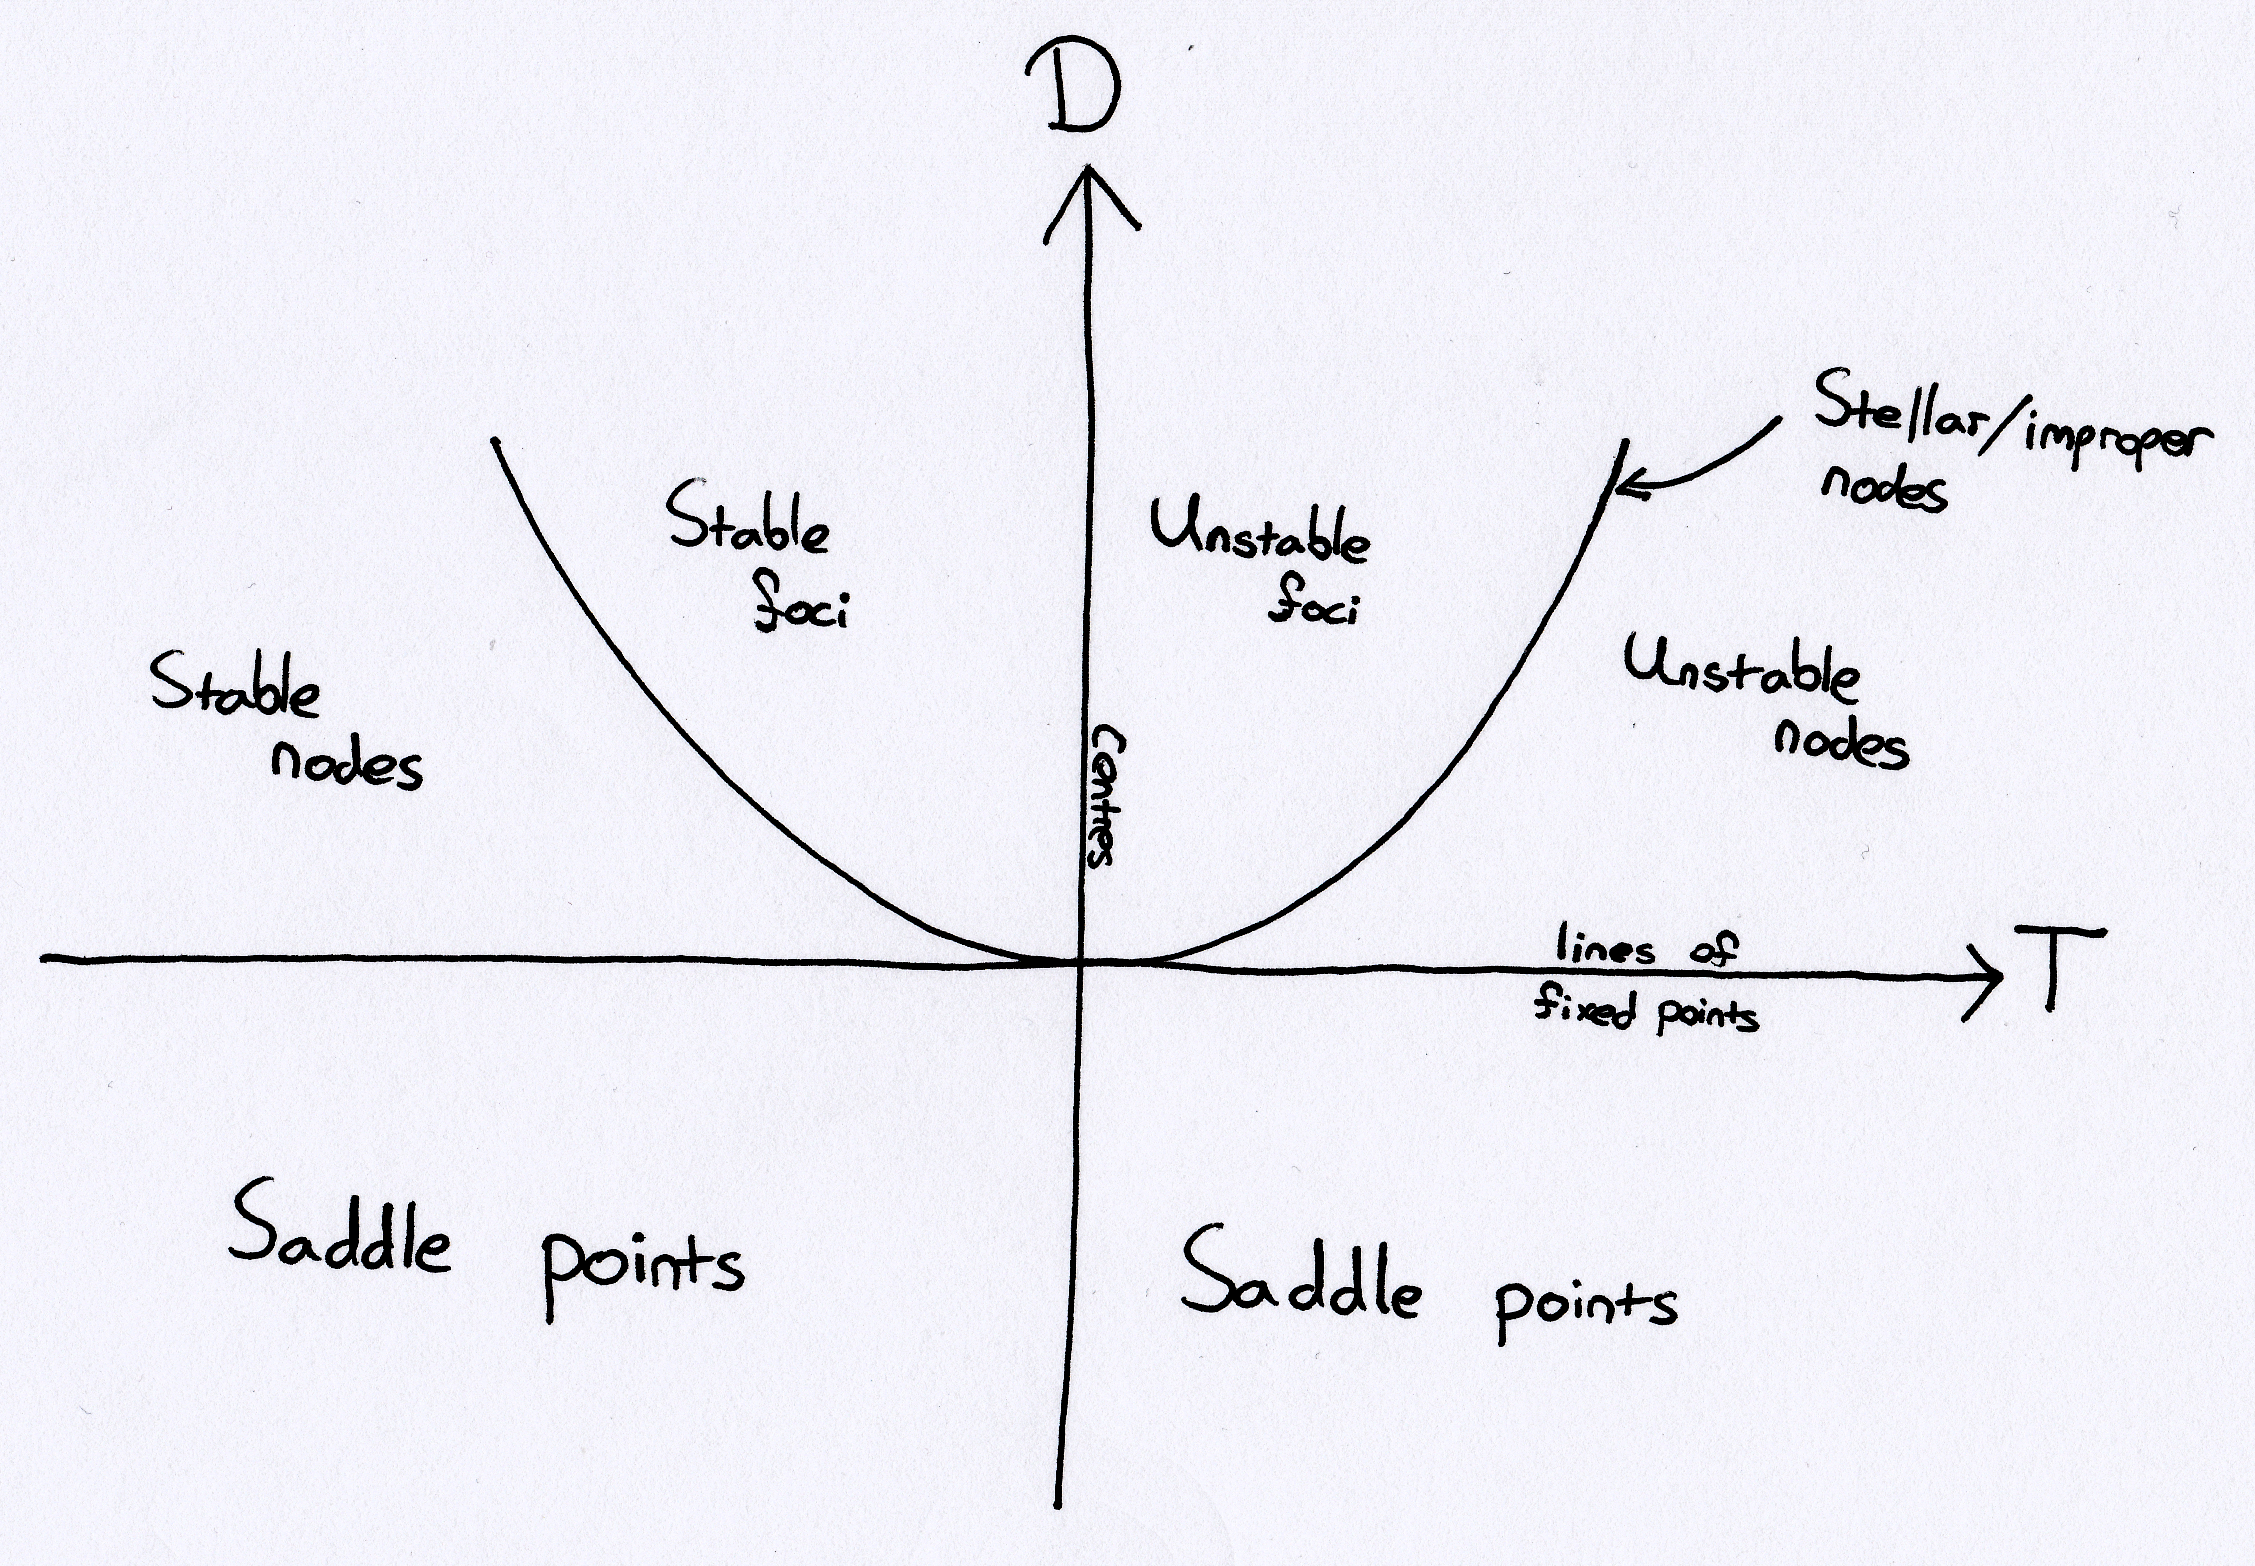
\includegraphics[width=14.4cm, height=10cm]{Diagram1.png}
\end{figure}
%
Notes:
\begin{enumerate}[(1)]
\item A Hamiltonian system is of the form
\[ \left( \begin{array}{c} \dot{x} \vspace{1mm}\\ \dot{y} \end{array} \right) =
\left( \begin{array}{r} \partial H / \partial y \vspace{1mm}\\ - \partial H / \partial x \end{array} \right) \]
for some $H(x,y)$. Fixed points are always saddles or centers because
\[ A = \left( \begin{array}{rr} H_{xy} & H_{yy} \\ -H_{xx} & -H_{xy} \end{array} \right) \implies T = 0 \]
Also $\dot{H} = \dot{\bm{x}}\cdot \nabla H = 0$ so the trajectories are
 (parts of) the contours of H.

\item The cannonical forms are obtained by using the eigenvectors $\bm{e}_i$ if
$\lambda _ i \in \mathbb{R}$ (possibly ``generalised'' for equal $\lambda$'s
and JNF, see Glendinning p 63) and $\mathrm{Re}(\bm{e}_1)$ and $\mathrm{Im}(\bm{e}_1)$ for 
$\lambda = \rho \pm i \omega$.

\item It is not necessary to change basis to classify the fixed point since
$T, \; D, \; \lambda$'s are invariant under $A \mapsto P^{-1}AP$, but knowing 
the eigenvectors may help sketch the phase diagram for the case of a saddle 
point.
\end{enumerate}
%
\textbf{Pertubation to A} (linear perturbations) 
\\
Cases (i)-(v) are robust - a small perturbation to A gives the same sort of 
eigenvalues and hence the same sort of fixed point.
\\
\\
Case (vi), if perturbed, may become a node or a focus, but these are 
topologically equivalent. The stability is not changed.
\\
\\
Cases (vii) and (viii) are fragile, - a small perturbation to (vii),
($\lambda = \pm i \omega$) may destroy the closed trajectories to give slow
spiralling inwards or outwards. A small perturbation to (viii) ($\lambda = 0$) 
may destroy the line of fixed points to give a slow drift towards/away from the
fixed point, and hence a saddle or node.
\\
\\
The fragility is because there are one or two eigenvalues on the border
Re$(\lambda) = 0$ between stability and instability.
\\
\\
\textbf{Definition:} Hyperbolic fixed point
\\
\\
A fixed point $\bm{x}_0$ of the system $\dot{\bm{x}} = \bm{f}(\bm{x})$ is a
hyperbolic fixed point if none of the eigenvalues $\lambda$ of the Jacobian
$ \left. \frac{\partial f_i}{\partial x_j} \right| _{\bm{x} = \bm{0}} $ satisfy
Re$(\lambda) = 0$, and is non-hyperbolic otherwise.
\\
\\
In n-dimensions $(n \geq 0)$ we classify a hyperbolic fixed point as
\begin{enumerate}[(i)]
\item a sink if all eigenvalues have Re $(\lambda) < 0$.
\item a source if all eigenvalues have Re $(\lambda) > 0$.
\item a saddle point otherwise (some $>0$, some $<0$)
\end{enumerate}
In 2D
\begin{center}
\includegraphics[scale = 0.15]{Diagram2.png}
\end{center}
% Diagram goes here!!
Non hyperbolic fixed points are important in bifurcation theory.
\\
\subsection{The effects of non-linear terms}
It is in fact true that the linearised system $\dot{\bm{y}} = A \bm{y}$
is essentially the same as the non linear system $\dot{\bm{x}} = \bm{f}(\bm{x})$
near a fixed point $\bm{x}_0$ provided
\begin{enumerate}[(i)]
\item The fixed point is hyperbolic
\item The non linear terms are $O( |\bm{x} - \bm{x}_0|^2)$
\end{enumerate}
(If (i) holds then the systems are topologically equivalent, if (ii) also holds,
then $\bm{h}(\bm{x})$ is a near identity map, so nodes are nodes and foci are
foci.)
\subsubsection{Stable and Unstable Manifold}
First, we formalise the idea of stable and unstable directions in the linearised
system.
\\
\\
\textbf{Definition:} The stable, unstable and center invariant subspaces of the
linearisation of $\bm{f}$ at a fixed point are the local linear subspaces.
\\
\\
$E^s, \; E^u, \; E^c$ spanned by the eigenvectors of the Jacobian, whose 
eigenvalues have real parts $<0$, $ >0$,  $=0$ respectively. (Generalised
eigenvectors for JNF)
\\
\\
For some types of fixed point, these spaces may be empty, e.g. for a hyperbolic
fixed point, $E^c$ is empty by definition.
\\
\\
Then we extend th linear picture into the non-linear domain for a hyperbolic
fixed point.
\\
\\
\textbf{Stable Manifold Theorem}
\\
If $\bm{0}$ is a hyperbolic fixed point of the system $\dot{\bm{x}} = \bm{f}(\bm{x})$,
with linear stable and unstable invariant subspaces $E^s$ and $E^u$ then in a 
sufficiently small neighbourhood of the origin, there exist local stable and
unstable manifolds
\begin{align*}
W^s_{loc}(\bm{0}) &= \{ \bm{x} : \bm{\phi}_t(\bm{x}) \to \bm{0} \mbox{ as } \
t \to \infty \} \\
W^u_{loc}(\bm{0}) &= \{ \bm{x} : \bm{\phi}_t(\bm{x}) \to \bm{0} \mbox{ as } \
t \to -\infty \} 
\end{align*}
these have the same dimension as $E^s$ and $E^u$ and are tangent to them
at $\bm{0}$.
\\
\\
Notes:
\begin{enumerate}[(1)]
\item For a saddle point in $\mathbb{R}^2$, this guarantees the existence of
two specific trajectories (the separatrices) that approach and leave the saddle.
\item For a sink this guarantees that all trajectories in some neighbourhood of the
sink tend to it
\item The local stable (unstable) manifolds can be extended to global 
stable (unstable) invariant manifolds $W^s \; (W^u)$ by following the flow 
backwards (forwards).
\end{enumerate}
The proof of this is not in the course - See Glendinning.
\\
\\
It is easy to calculate approximations to $W^s$ and $W^u$ for a saddle point
in $\mathbb{R}^2$.
\\
\\
Wlog (Change of origin and basis) assume that the saddle is at $\bm{x}=\bm{0}$
and that $E^s$ is $x=0$ and $E^u$ is $y=0$.
\\
\\
\begin{tabular}{ m{4.5cm} m{9cm}  } 
\includegraphics[scale = 0.15]{fig14.png}  & 

Then $W^s_{loc}$ becomes $x = S(y)$ with $S(0) =0, \; S'(0)=0$ 
$W^u_{loc}$ is $y = U(x)$ with $U(0) =0, \; U'(0)=0$.
\end{tabular}
\\
Since $W^s$ and $W^u$ are invariant,
\\
\[
 \left. \dot{x}\right|_{(S,y)} = \frac{dS}{dy} \left.\dot{y}\right|_{(S,y)} \qquad \qquad
 \left.\dot{y}\right|_{(x,U)} = \frac{dU}{dx} \left.\dot{y}\right|_{(x,U)}
\]
\\
\textbf{Example:} 
\[ \left( \begin{array}{c} \dot{x} \\ \dot{y} \end{array} \right) = 
\left( \begin{array}{c} x - xy \\ -y+x^2 \end{array} \right) \qquad \qquad
A|_{\bm{x} = \bm{0}} = \left( \begin{array}{cr} 1 & 0 \\ 0 & -1 \end{array} \right) \]
Assume that
\[ y = U(x) = a_2 x^2 + a_3 x^3 + a_4 x^4 + \dots \]
substitute into 
\[ \dot{y} = U'\dot{x}  \implies -(a_2x^2+a_3x^3 + a_4x^4 + \dots) + x^2 
= (2a_2x + 3a_3x^2 + 4a_4x^3 + \dots)(x - a_2x^3 - \dots ) \]
Equate coefficients:
\begin{align*}
a_2 &= \frac{1}{3} \\
a_3 &= 0 \\
a_4 &= \frac{2}{45} \quad \mbox{etc.}
\end{align*}
Locally for $|\bm{x}| \ll 1$ \\
\begin{center}
\includegraphics[scale = 0.15]{Diagram3.png}
\end{center}
In higher dimensions, would write $\bm{y} = \bm{U}(\bm{x})$ and solve
\[ \dot{y}_i = \frac{\partial U_i}{\partial x_i} \dot{x_j} \]
Where the $x_j$'s span $E^u$ and the $y_i$'s span $E^s$.
\subsubsection{Non-Linear terms in non-hyperbolic cases}
There are many possibilities depending on the non-linear terms.
\begin{enumerate}[(a)]
\item $\lambda = \pm i \omega$ Linear system is a centre. Are the trajectories
really closed?
\\
\\
\textbf{Example:}
\[ \left. \begin{array}{lr} 
				\dot{x} = & - y \pm x^3 \\
				\dot{y} = & x \pm y^3
\end{array} \right\} \implies \begin{array}{lr}
				\dot{r} = \pm \frac{x^4+y^4}{r} \\
			\dot{\theta} = 1 \pm \frac{xy^3-yx^3}{r^2} \end{array}\]
Now as $r \to 0$, $\dot{\theta} \to 1$. Thus the system is a stable focus if we choose '+'
and an unstable focus if we choose '$-$'.
\\
\\
\textbf{Example:}
\begin{alignat*}{4} 
& \dot{x} &&=  - && y - 2yx^2 =  &&\frac{\partial H}{\partial y} \\
& \dot{y} &&=    && x + 2xy^2 = -&&\frac{\partial H}{\partial x} 
\end{alignat*} 
for $H = - \frac{x^2+y^2}{2} - x^2y^2$. 
The trajectories are contours of H, which are closed near the maximum at 
$\bm{0}$. So the fixed point really is a non-linear centre with nested 
periodic orbits.
%
\item $\lambda_1 = 0$, $\lambda_2 \neq 0$. Which way does the system drift 
along $\bm{e}_1$?
\\
\\
\textbf{Example:} \\ 
\begin{center}
\begin{tabular}{ m{3cm} m{3cm} m{3cm}  } 
$\begin{array}{lr}
 \dot{x} = & x^2 \\
 \dot{y} = & -y \end{array}$
& \includegraphics[scale=0.1]{fig15.png}
& Saddle-node \\ 
\\
\\
$\begin{array}{lr}
 \dot{x} = & x^3 \\
 \dot{y} = & -y \end{array}$
& \includegraphics[scale=0.1]{fig15.png}
& Non-linear saddle
\end{tabular}
\end{center}
\item $\lambda_1 = \lambda_2 = 0$. Ad hoc methods needed.
\\
\\
In some cases, it is useful to switch to polars and consider the sign of
$\dot{r}$ and $\dot{\theta}$ as $r \to 0$.
\\
\\
\textbf{Example:} $\dot{\theta} >0$ \\
\begin{center}
\includegraphics[scale = 0.15]{fig17.png} \\
\includegraphics[scale = 0.16]{fig18.png}
\end{center}
In nastier cases, the curves $\dot{\theta} = 0$ can form a cusp.
\begin{center}
\includegraphics[scale = 0.16]{fig19.png}
\end{center}
\end{enumerate}
%
%
\subsection{Sketching phase planes/portraits}
%
\textbf{Example:}
\\
\begin{align*}
\dot{x} &= x(1-y) \\
\dot{y} &= -y + x^2
\end{align*}
This has fixed points at $(0,0)$ and at $(\pm1,1)$. 
\begin{center}
\begin{tabular}{ m{2cm} m{3cm} m{3cm} }
$(0,0)$ & $A = \left( \begin{array}{cr} 1 & 0 \\ 0 & -1 \end{array} \right)$ & saddle point \\ \\ \\
$(\pm 1,1)$ & $A = \left( \begin{array}{cr} 0 & \mp 1 \\ \pm 2 & -1 \end{array} \right)$ & stable foci
\end{tabular}
\end{center}
It is clear why $(0,0)$ is a saddle point. For $(\pm1,1)$ observe that 
$T=-1$, $D=2$, $T^2 < 4D$, and therefore $(\pm 1, 1)$ are stable foci. Before
sketching, observe that.
\begin{itemize}
\item $x = 0$ is a trajectory.
\item $\dot{x}=0$ on $y=1$
\item $\dot{y} = 0$ on $y=x^2$
\item $\dot{y} \,\, ^{<}_{>} \,\, 0$ if $y \,\,^{<}_{>} \,\, x^2$
\item Symmetry in y axis; under $x \mapsto -x$, $\dot{x} \mapsto -\dot{x}$, and $\dot{y} \mapsto \dot{y}$
\item Know that the unstable manifold is given by $y \approx \frac{1}{3} x^2 + \frac{2}{45} x^4$
near $x=0$ (See earlier example)
\end{itemize}
Put all of this together to sketch the following:
\begin{figure}[H]
\centering
\includegraphics[scale=0.2]{fig20.png}
\end{figure}
\noindent In general, here are some steps to follow when sketching a phase plane.
\begin{enumerate}[1.]
\item Find the fixed points.
\item \begin{enumerate}[(a)] \item Calculate the Jacobian to find the kind of eigenvalues and classify
				the fixed points.
				\item If any are non-hyperbolic, consider non-linear terms, possible
				Hamiltonian structure, signs of $\dot{x}$, $\dot{y}$, $\dot{r}$ or 
				$\dot{\theta}$ as $|\bm{x} - \bm{x}_0| \to 0$.
      \end{enumerate}
\item Calculate the eigenvectors for saddles.
\item Consider the sign of $\dot{x}$ and $\dot{y}$ - the curves where these are
zero are called nullclines.
\item Construct the global picture by joining up the local behaviour near fixed
points. (especially the separatrices of saddles) using the arrows from $\dot{x}$
and $\dot{y}$.
\item At some stage, decide whether there are periodic orbits.
\end{enumerate}
%
%
%
\section{Stability}
\subsection{Definitions}
It is clear what it means for a hyperbolic node or focus to be stable, but we
ned to be more careful with the stability of other kinds of fixed points or 
invariand sets, because there are at least two notions of stability.
\\
\\
\textbf{Definition:} Lyapunov stability
\\
A fixed point $\bm{x}_0$ of a flow $\bm{\phi}_t$ is Lyapunov stable if
$\forall \epsilon > 0, \; \exists \delta > 0$ s.t. $|\bm{x}-\bm{x}_0| < \delta$
$\implies |\bm{\phi}_t(\bm{x}) - \bm{x}_0| < \epsilon$ $\forall t>0$.
A motto is ``Start near, stay near'' stability.
\\
\\
\textbf{Definition:} Quasi-asymptotic stability (QAS)
\\
A fixed point $\bm{x}_0$ of a flow $\bm{\phi}_t$ is quasi-asymptotically 
stable if $\exists \delta > 0$ s.t. $|\bm{x}-\bm{x}_0| < \delta$ $\implies
\bm{\phi}_t(\bm{x}) \to \bm{x}_0$ as $t \to \infty$.
\\
\\
These are not the same!
\\
\\
\textbf{Example:}
\\
\begin{tabular}{m{3cm} m{4cm} m{9cm}  } 
$\begin{array}{lr} 
\dot{r} = & 0 \\
\dot{\theta} = & 1
\end{array}$ &
\includegraphics[scale = 0.15]{fig11.png}  & 
Lyapunov stable, but not asyptotically stable.
\\
\\
$\begin{array}{lr} 
\dot{r} = & r(1-r^2) \\
\dot{\theta} = & \sin^2(\theta/2)
\end{array}$ &
\includegraphics[scale = 0.15]{fig14.png}  & 
The point $r=1$, $\theta = 0$ is QAS but not Lyapunov stable
\end{tabular}
\\
\\
\textbf{Definition:} Asymptotic stability (AS)
\\
A fixed point $\bm{x}_0$ is asymptotically stable if it is both Lyapunov stable
and quasi-asymptotically stable.
\\
\\
\textbf{Example:} A sink (Re $\lambda_i <0 \; \forall \, i$) is asymptotically
stable. (Choose $\delta$ sufficiently small that the linear terms dominate)
A saddle or source is obviously not Lyapunov stable, hence not AS.
\\
\\
For other kinds of invariant sets $\Lambda$ e.g. limit cycles, define
\[ N_{\delta}(\Lambda) = \{ \bm{x} : \exists \bm{y} \in \Lambda \mbox{ with } \
|\bm{x} - \bm{y}| < \delta \} \]
and say 
\[ \bm{\phi}_t(\bm{x}) \to \Lambda\]
if
\[\min_{\bm{y} \in \Lambda} \
\{ | \bm{\phi}_t(\bm{x}) - \bm{y}| \} \to 0 \quad \mbox{ as } \quad t \to \infty \]
\\
Then say $\Lambda$ is Lyapunov stable if $\forall \epsilon > 0$ $\exists \delta>0$ s.t.
$\bm{x} \in N_{\delta}(\Lambda) \implies \bm{\phi}_t(\bm{x}) \in N_{\epsilon}(\Lambda)$
$\forall t >0$.
\\
\\
Say $\Lambda$ is QAS if $\exists \delta >0$ s.t. $\bm{x} \in N_{\delta}(\Lambda) \implies \
\bm{\phi}_t(\bm{x}) \to \Lambda$ as $t \to \infty$.
\\
\\
Say $\Lambda$ is AS if it is both LS and QAS.
\\
\subsection{Lyapunov functions}

\end{document}
